%%

\begin{frame}
	\frametitle{ABI исполняемых файлов в Linux}

	\begin{block}{Форматы исполняемых файлов}
		\begin{itemize}
			\item {\tt a.out} -- начало Unix
			\item {\tt COFF} -- Common Object File Format -- историческое продолжение {\tt a.out}
			\item {\tt ELF} -- Executable and Linkable Format -- настоящее Unix-like систем
		\end{itemize}
	\end{block}
\end{frame}

\begin{frame}
	\frametitle{ELF}
	\begin{columns}
		\column{0.5\textwidth}
			\begin{block}{Executable and Linkable Format}
				Файлы могут включать:
				\begin{itemize}
					\item Таблицу Program Header,  описывающую ноль или более сегментов
					\item Таблицу Section Header,  описывающую ноль или более секций
					\item Данные,  упомянутые в записях названных таблиц
				\end{itemize}
			\end{block}
		\column{0.5\textwidth}
			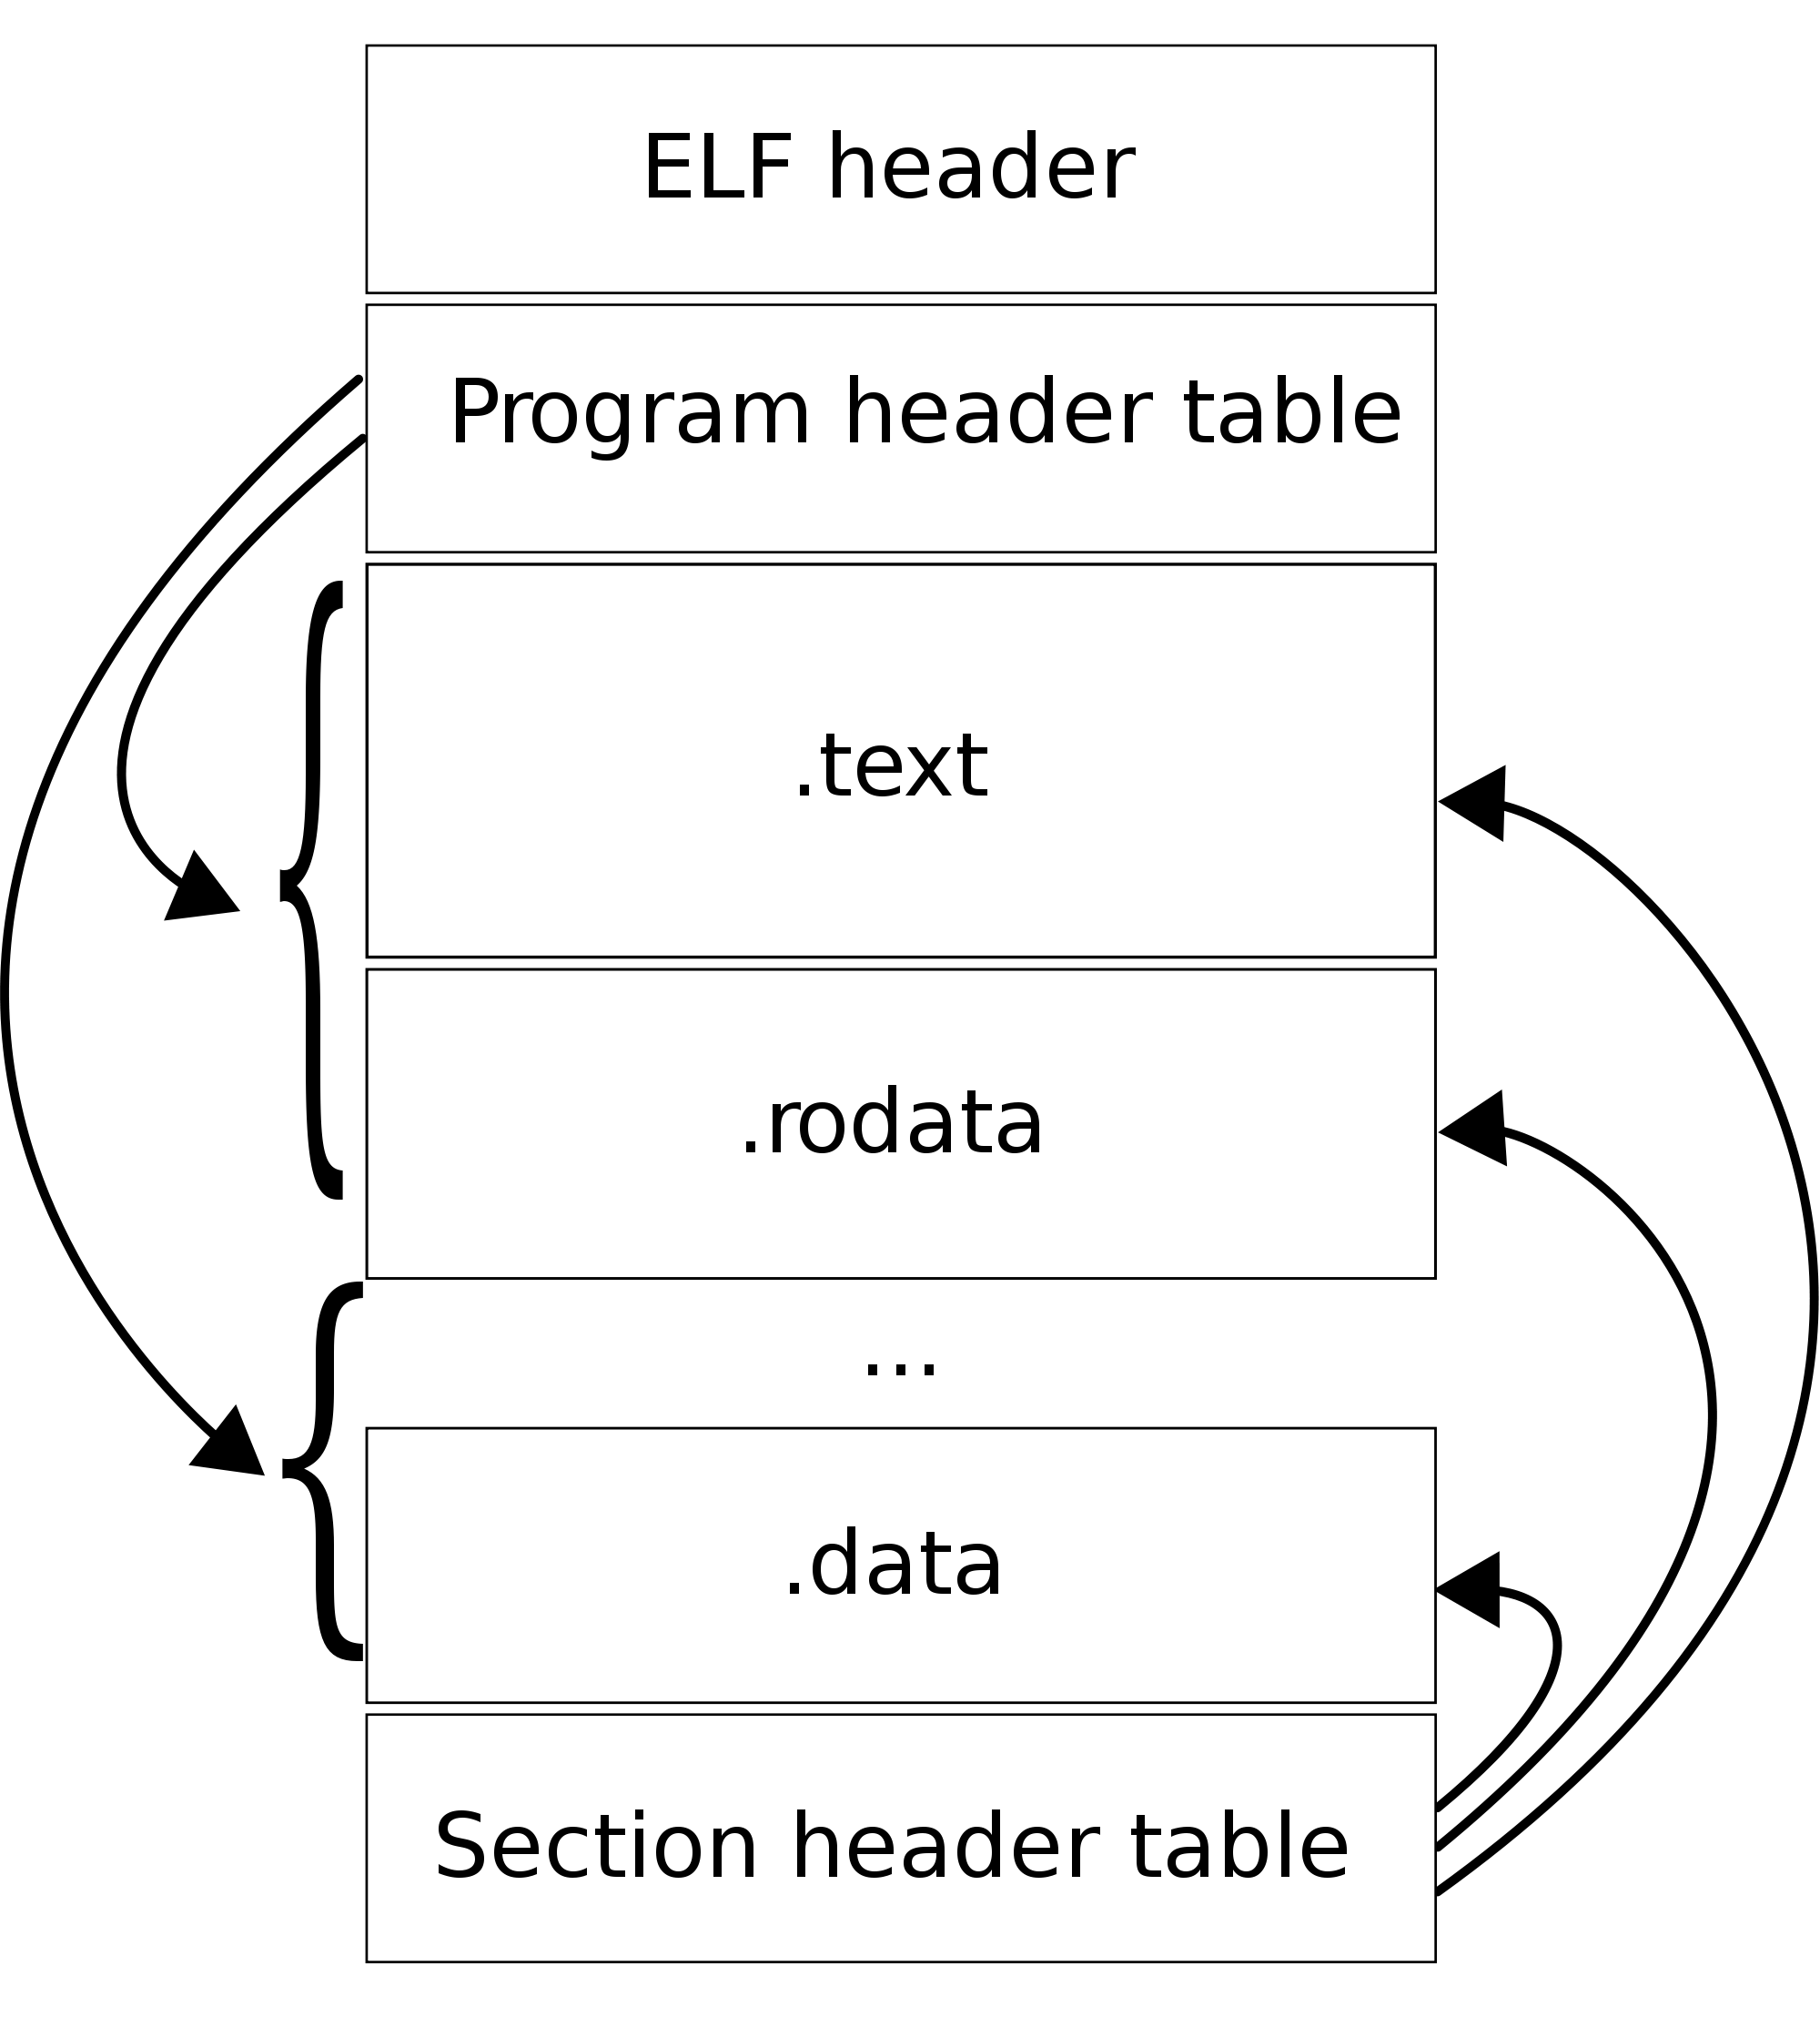
\includegraphics[height=0.8\textheight]{../../slides/elf-analysis/Elf-layout.png}
	\end{columns}
\end{frame}

\begin{frame}
	\frametitle{}

	\begin{block}{Пример}
		Для анализа понадобится пример из занятия по введению в gcc (последовательность линковки библиотек).
	\end{block}

	Пример доступен по адресу \url{https://github.com/d4s/linux\_courses/tree/master/epam/examples/make/linking}
	
\end{frame}

\begin{frame}
	\frametitle{Структура ELF-файла}

	\begin{block}{readelf}
		Утилита для просмотра информации файлов в формате ELF.
	\end{block}

	\pause

	\begin{block}{Упражнение: просмотр программных заголовков}
		\begin{itemize}
			\item {\tt readelf -{}-file-header main-A\_B} -- интерпретация заголовка ELF-файла
			\item {\tt readelf -{}-sections main-A\_B} -- перечисление секций (для линковки)
			\item {\tt readelf -{}-segments main-A\_B} -- 
				перечисление программных сегментов (для исполнения)
			\item {\tt readelf -{}-symbols main-A\_B} -- список таблицы символов
		\end{itemize}
	\end{block}
\end{frame}

\begin{frame}
	\frametitle{Таблица символов}

	\begin{block}{strings}
		Утилита для получения символов из ELF-файла.
	\end{block}

	\begin{block}{nm}
		Утилита для получения символов из object файла.
	\end{block}

	\begin{block}{strip}
		Утилита для удаления символов из object файла.
	\end{block}
\end{frame}

\begin{frame}
	\frametitle{Таблица символов}

	\begin{block}{Упражнение}
		\begin{enumerate}
			\item {\tt strings main-A\_B}
			\item {\tt nm main-A\_B}
			\item {\tt nm -u main-A\_B}
			\item {\tt ls -l main-A\_B}
			\item {\tt strip main-A\_B}
			\item {\tt ls -l main-A\_B}
			\item {\tt nm main-A\_B}
			\item {\tt повторить предыдущее упражнение}
			\item Сделать выводы
		\end{enumerate}
	\end{block}

\end{frame}

